

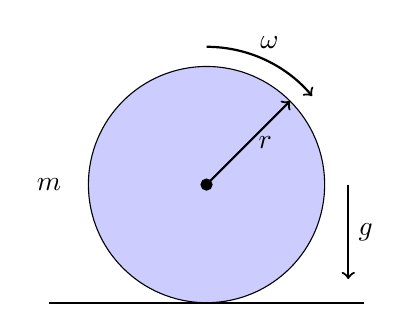
\begin{tikzpicture}
    % Draw the disc
    \fill[blue!20] (0,0) circle (1.5cm); % Circle with light blue fill
    \draw (0,0) circle (1.5cm); % Outer circle for the disc
    
    % Center and radius line
    \draw[->, thick] (0,0) -- (45:1.5cm) node[midway, right] {$r$};
    \draw[fill=black] (0,0) circle (2pt); % Center dot

    % Mass label
    \node at (-2, 0) {$m$};

    % Angular velocity arrow
    \draw[->, thick] (0,1.75) arc[start angle=90, end angle=40, radius=1.75cm];
    \node at (0.8,1.8) {$\omega$};
    
    % Ground line
    \draw[thick] (-2, -1.5) -- (2, -1.5); % Horizontal ground line
    
    % Gravity arrow
    \draw[->, thick] (1.8,0) -- (1.8, -1.2) node[midway, right] {$g$};

\end{tikzpicture}

